\chapter{System Bandwidth Comparison}


In figures \ref{fig:speedup} and \ref{fig:speedup2} we presented an overview for performance of the GPU version of SCEPTIC3D on two distinct systems. System 1 consisted of an Intel(R) Core i7 930 quad core processor clocked at 2.8GHz and two EVGA GTX 470 graphics cards. System 2 consisted of two Intel(R) Xeon(R) E5420 quad core processors clocked at 2.53GHz and one EVGA GTX 590. In figure \ref{fig:speedup2} the speedup factors for the GPU version vs the CPU version were much higher on system 2. There are two reasons for this. The first reason is that the GPU in system 2, the GTX 590, is more powerful than the two GTX 470's in system 1. The second reason has to do with the difference in memory bandwidth between the two systems.

\noindent \begin{figure}
\begin{center}
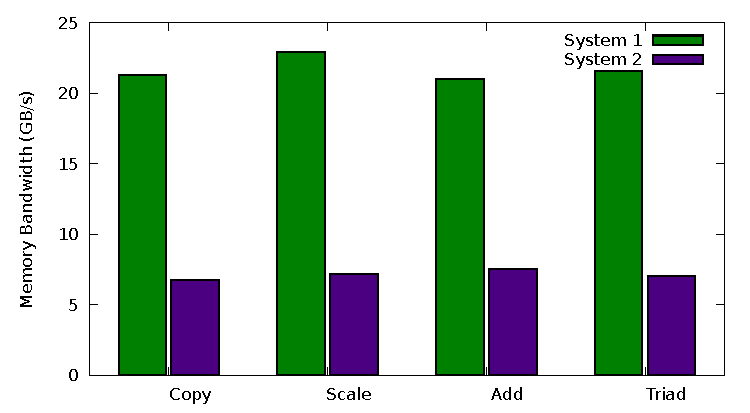
\includegraphics[width=6in]{appb/bandwidth_test.pdf}
\end{center}
\caption[System Memory Bandwidth Comparison]{System memory bandwidth comparison for the two test systems used to generate the results in \ref{fig:speedup} and \ref{fig:speedup2}.}
\label{fig:memory_bandwidth_compare} 
\end{figure} 

In figure \ref{fig:memory_bandwidth_compare} we performed four vector operations on 20 million element arrays. These vector operations consisted of a simple copy $B = A$, a scalar multiply $B = \alpha A$, a vector add $C = A+B$, and a triad $C = B+\alpha A$. MPI was used to run one copy of the each operation for every core on the target system, the MPI threads were synchronized between operations. Run times were recorded for 50 iterations of the vector operations, the run time at each iteration is the mean of the individual thread run times. The memory bandwidth of each operation is calculated as the number of bytes read and written divided by the minimum run time.    



\clearpage
\newpage
